% --------------------------------------------------------------------

\textbf{Huomautuksia arvioijalle}

Symbolilla --> merkitsemäni kohdat ovat ideoita sisällöstä. Näiden olisi
kuitenkin tarkoitus kuvata lopullista sisältöä, eli niiden kuuluu olla
loogisessa järjestyksessä ja muutenkin olla järkeviä.

Olen merkinnyt kulmasulkeilla < > viitteet jotka toistaiseksi puuttuu lähteistä.

Olen pyrkinyt muotoilemaan uusiksi kaikki kohdat jossa oli käytetty ensimmäistä
personamuotoa. Sitä ei pitäisi enää esiintyä.

\newpage

\section{Johdanto}

Ohjelmistoalan kilpailutilanteen kiristyessä yritykset etsivät jatkuvasti tapoja
tehostaa toimintaansa. Ketterien menetelmien on todettu parantavan tehokkuutta
sekä laatua \citeppri{Livermore2008}, mikä nostaa ne houkuttelevaksi vaihtoehdoksi
tehostamista tavoitteleville yrityksille. Ketterien menetelmien käyttöönotto on
kuitenkin haastavaa suurissa yrityksissä \citeppri{Dyba2009}. Alun perin pieniin
projekteihin ja tiimeihin\footnote{Tässä työssä käytetään ohjelmistoalalla
vakiintunutta lainasanaa tiimi (engl. team) viitaten projektin työryhmään.}
suunnitellut mallit ovat osoittautuneet vaikeiksi soveltaa suuremmassa
mittakaavassa \citeppri{Boehm2005}.

Suuret yritykset toimivat usein perinteisten ohjelmistotuotannon mallien
mukaisesti. Nämä mallit pyrkivät optimoimaan toimintaa tarkalla suunnittelulla
ja prosessien määrittelyllä. Tämänlainen lähtökohta soveltuu kuitenkin huonosti
ohjelmistokehitykseen, sillä kehitysprojekteissa tulee lähes poikkeuksetta
tilanteita, joita on mahdotonta tai liian työlästä ennustaa \citeppri{Schwaber2002}.
Suurimpia ongelmia suunnitelmavetoisissa menetelmissä on vaatimusten muuttamisen
korkea hinta sekä myöhäinen palaute tuotteen laadusta \citeppri{Petersen2010}.
Pitkät julkaisuvälit, muutoksiin vastaamisen kalleus sekä etäisyys asiakkaista
heikentävät yritysten kilpailukykyä. Apua näihin ongelmiin toivotaan löytyvän
ketterien kehitysmallien soveltamisella.

Tämän työn tavoite on esittää nykyinen tutkimuksen tila ketterien
ohjelmistokehitysmenetelmien käyttöönotosta suurissa organisaatioissa,
tarkastellen erityisesti siihen liittyvää organisaatiomuutosta. Ketterien
menetelmien käyttöönotosta on olemassa tutkimuksia, mutta ne keskittyvät
enimmäkseen pieniin organisaatioihin tai yksittäisiin tiimeihin. Suuret
organisaatiot mukautuvat uusiin menetelmiin hitaammin, mikä voidaan olettaa
syyksi siihen, että laajaa tutkimusta suuren mittakaavan ketterästä muutoksesta
ei ole aikaisemmin tehty.

Tämä työ on toteutettu mukaillen järjestelmällisen kirjallisuustutkimuksen
muotoa, kartoittaen olemassa olevat tapaustutkimukset ja kokemusraportit.
Tutkimuskysymys johon tässä työssä vastataan on: Mitkä tekijät vaikuttavat
ketterän kehitysmallin organisaatiomuutoksen läpiviemiseen isossa
organisaatiossa? Työn tulos osoittaa, että ketterien kehitysmenetelmien
käyttöönotosta isoissa organisaatioissa on olemassa riittävästi ensisijaisia
tutkimuksia kirjallisuustutkimukseen.

Luvussa \ref{sec:tausta} esitellään aikaisempia tutkimuksia liittyen tämän työn
aihealueeseen, sekä todetaan, että työ vastaa olemassa olevaan aukkoon
tutkimuksessa. Luvussa \ref{sec:menetelma} on esitelty järjestelmällisen
kirjallisuustutkimuksen menetelmä, sekä tapa jolla sitä on sovellettu tämän
kandidaatintyön kokeellisena osiona. Luvussa \ref{sec:tulokset} käsitellään
kirjallisuustutkimuksen tulokset. Lopuksi esitellään tuloksista tehdyt
johtopäätökset sekä työn yhteenveto.


% --------------------------------------------------------------------
\clearpage
\section{Työn taustat}
\label{sec:tausta}

Tämän työn tavoitteena on kuvata perusteita, haasteita ja menestyksen tekijöitä
ketterien kehitysmenetelmien käyttöönoton suurissa organisaatioissa.
Taustatietona työlle tässä luvussa esitellään havaintoja edellisistä
tutkimuksista jotka liittyvät ketterien menetelmien käyttöönotton haasteisiin,
sekä suuren mittakaavan ketterään kehitykseen. Myös ketterien menetelmien
menestyksekkään käyttöönotton tekijöitä esitellään. Luvun lopuksi perustellaan
tämän työn merkitys suhteessa olemassa olevaan tutkimuskeen.

\subsection{Ketterä ohjelmistokehitys}

Ketterä ohjelmistokehitys on joukko menetelmiä jotka on kehitetty vaihtoehdoksi
niin kutsutulle perinteiselle suunnitelmavetoiselle kehitykselle. Ketterien
menetelmien näkökulmasta perinteiset mallit pyrkivät vähentämään muutoksia
tuotteen kehityksessä, ja tulkitsevat muutoksia virheinä. Tuotteen
mukautumiskyky kehityskaaren aikana ja kyky vastata arvaamattoman maailman
haasteisiin ovat nykyään kuitenkin kriittisiä tekijöitä. Muutoksen omaksuminen
kehityksessä, korkean laadun tavoitteleminen ensi askelista alkaen, sekä
ihmiskeskeisyys ovat ketterien menetelmien keskeisiä teemoja.
\citeppri{Highsmith2001}

Ketterää kehitystä on sekä kritisoitu että puollettu, ja tutkimukset ovat
osoittaneet muutoksen omaksumisen sekä menestyksen että epäonnistumisen
tekijöinä \citeppri{Boehm2002}. On osoitettu, että ketterät menetelmät ovat
parantaneet sekä kehittäjien että asiakkaiden tyytyväisyyttä, mutta toisaalta on
olemassa todisteita siitä, että ketterät menetelmät eivät välttämättä sovellu
suuriin hankkeisiin \citeppri{Dyba2009}. \citepri{Boehm2002} ehdottaakin, että
organisaatioiden tulisi etsiä itselleen sopiva tasapaino suunnitelmavetoisten ja
ketterien menetelmien välillä.

Nykyään yleisiä ketterän kehityksen menetelmiä ovat Scrum ja Extreme Programming
(XP) \citeppri{Dyba2008}. Scrum on projekinhallintamenetelmä, joka painottaa
tiimikeskeistä toimintaa, ajallista rytmittämistä (time-boxing), jatkuvaa
edistymisen seurantaa, sekä asiakaskeskeisyyttä \citeppri{Schwaber2002}.
XP-menetelmä perustuu kokoelmaan käytäntöjä, joista keskeisimmät ovat jatkuva
palaute kehityksestä, testausvetoinen kehitys, asiakkaan jatkuva mukanaolo,
pariohjelmointi ja jatkuva yhdentäminen (engl. Continuous Integration
CI) \citeppri{Beck1999}.

--> Kevyt kehitysmalli (engl. lean development)

\subsection{Ketterien menetelmien käyttöönoton haasteita}

Ketterien menetelmien käyttöönotto ei perustu yksittäisiin uusiin
toimintatapoihin tai työkaluihin, vaan kokonaisvaltaiseen toiminta- ja
ajattelutavan muutokseen. Tämänlainen muutos vaatii koko organisaatiokulttuurin
muuttumista \citeppri{Misra2009}, mikä on haastavampaa kuin pelkästään uusien
työkalujen käytön opetteleminen. Muutosta saattaa vaikeuttaa
suunnitelmavetoiseen toimintamalliin juurtuneet ajattelutavat ja asenteeet
\citeppri{Mahanti2006,Nerur2005}. Ketterässä kehityksessä organisaatiokulttuurin
on oltava tiimi- ja asiakaskeskeinen, tiimeillä pitää olla valinnanvapaus
työkalujen ja menetelmien käytössä ja tiedon välittyminen pitää mahdollistaa
myös muissa muodoissa kuin kirjoitettuna dokumentaationa \citeppri{Misra2009}.

Kehittäjät ovat keskeisessä roolissa ketterissä malleissa. Organisaatiossa
joissa on vahva tausta suunnitelmavetoisesta kehityksestä saattaa kehittäjien
osaaminen olla kapea-alaista, mikä muodostuu ongelmaksi ketterien menetelminen
vaatiessa enemmän yleisiä taitoja \citeppri{Nerur2005}. Keskeinen ominaisuus
jota kehittäjien tulisi osoittaa ketterissä malleissa on itseohjautuvuus
\citeppri{Misra2009}. Ketterien menetelmien yhteydessä on suositeltu keskivertoa
parempien kehittäjen käyttämistä \citeppri{Boehm2002}. Pelkästään
huippukehittäjien käyttäminen ei ole välttämätöntä, mutta heikoimpien
suoriutujien mukanaolo on haitallista ketterässä kehityksessä
\citeppri{Nerur2005,Boehm2005}. Muutoksen myötä kehittäjien on omaksuttava uusia
työtapoja, mikä saattaa aiheuttaa muutosvastarintaa. Eräitä syitä
muutosvastarintaan voivat olla pelko omien taitojen riittämättömyydestä uudessa
ympäristössä tai kateuden tunne työtovereiden uusista tehtävistä
\citeppri{Boehm2005}.

Tiimien prosessien lisäksi myös liiketoiminnan prosesseja joudutaan sopeuttamaan
ketteriin menetelmiin. Tuotannon ja suunnittelun tulisi etääntyä
elinkaariajattelusta ja painottaa iteratiivista ja toiminnallisuuksiin
keskittyvää mallia \citeppri{Nerur2005}. Ongelmana on, että perinteisissä
malleissa on annettu pitkän aikavälin suunnitelmia ja tehty sitoomuksia, mutta
ketterät menetelmät perustuvat nopeiden muutosten mahdollistamiseen. Tämän takia
organisaation johdon on hyväksyttävä muutosten tekeminen lyhyemmällä
aikajänteellä \citeppri{Misra2009}. Perinteisesti liiketoimintaa on ohjattu
pitkän tähtäimen suunnittelulla, mutta ketterät menetelmät painottavat, että
merkityksellistä suunnittelua voi tehdä vain lähitulevaisuuteen
\citeppri{Boehm2005}. Johdon on myös hyväksyttävä, että kehitystyötä ei kannata
pyrkiä hallitsemaan yksityiskohtaisella tasolla, vaan sallittava esimerkiksi
kevyemmät raportointikäytännöt \citeppri{Cohn2003}.

Ketterät menetelmät vaativat asiakkaan vahvempaa läsnäoloa, mutta kaikki
asiakkaat eivät halua tai voi osallistua kehitykseen \citeppri{Nerur2005}.
Muodollisten dokumenttien puuttuessa asiakkailta vaaditaan luottamusta
kehitystiimiin, sekä joustavuutta neuvoteltaessa mahdollisista muutoksista
\citeppri{Misra2009}. Myös sopimuskäytäntöjä pitää muuttaa perustumaan toimivan
ohjelmiston toimittamiseen sen sijaan, että keskitytään muodollisiin
katselmointeihin tai dokumentaatioon \citeppri{Boehm2005}.

Suurissa organisaatioissa ketterien menetelmien käyttöönotto on haastavampaa
kuin pienissä \citeppri{Livermore2008,Dyba2008}. Tärkeä tekijä suurissa
organisaatioissa on se, että projektit ovat harvoin riippumattomia toisista.
Riippuvuudet kasvattavat tiimin tarvetta kommunikoida ulospäin. Suuri mittakaava
saattaa pakottaa ketteryyden vähentämistä esimerkiksi muodollisen dokumentaation
lisäämisellä \citeppri{Lindvall2004}. Ketterät menetelmät saattavat myös joutua
törmäyskurssille organisaation muiden toimintojen kanssa. Muun muassa
henkilöstöhallinnon käytännöt saattavat estää työntekijöitä ottamasta uusia ja
laajempia rooleja, mitä ketterä kehitys vaatii \citeppri{Boehm2005}.
Muutoksenhallintalautakunta (engl. change control board, CCB) saattaa
hankaloittaa refaktoroinnin ja jatkuvan yhdentämisen käyttöä
\citeppri{Lindvall2004}. Organisaation kehitystyöhön liittymättömiä toimintoja
pitää informoida muutoksesta ketterään kehitykseen, ja ketterää mallia pitää
sovittaa toimimaan yhteen niiden kanssa
\citeppri{Lindvall2004,Cohn2003,Boehm2005}. Liittyminen ympäröivään
organisaatioon saattaa tulla sillä kustannuksella, että on tuettava
lopputuotteen kannalta vähemmän arvoa lisääviä käytäntöjä, kuten dokumentaatiota
ja jäykempää suunnittelua \citeppri{Mahanti2006}.

\subsection{Menestyksekkään käyttöönoton tekijöitä}

Ketterien menetelmien käyttöönottossa kannattaa seurata organisaatiomuutoksiin
yleisesti liittyviä hyviä käytäntöjä. Näitä ovat johdon myötämielisyys
muutokseen, pilottiprojektien käyttö, sekä henkilöstön kouluttaminen.

Johdon myötämielisyydellä ja osallistumisella on merkittävä vaikutus
onnistumiseen kun muutetaan ohjelmistokehityksen toimintatapoja
\citeppri{Livermore2008}. Ketterän kehityksen lupaama tehokkuuden kasvu
houkuttelee johtoa tukemaan ketterien menetelmien käyttöönottoa, erityisesti jos
aikaisempien projektien on havaittu ylittäneen budjetteja tai aikarajoja
\citeppri{Cohn2003}. Käyttöönoton riskejä on järkevää vähentää kokeilemalla
ketteriä menetelmiä lyhyiden pilottiprojektien kautta \citeppri{Lindvall2004}.
Onnistunut pilottiprojekti vahvistaa johdon tukea ketterän kehityksen
jatkamiselle, ja projektitiimi saa arvokkasta kokemusta ketterien menetelmien
soveltamisesta, jota voidaan hyödyntää kähyttöönoton laajentuessa
\citeppri{Mahanti2006}.

Uusien menetelmien käytön koulutus on oleellinen tekijä ketterien menetelmien
menestyksekkäässä käyttöönotossa \citeppri{Livermore2008}. Koulutus auttaa
kitkemään muutosvastarintaa ja väärinkäsityksiä, mikä on erityisen tärkeää,
sillä ketterä kehitys perustuu sujuvaan ihmisten väliseen kommunikaatioon
\citeppri{Mahanti2006}. Koulutus ei koske pelkästään kehittäjiä, vaan
organisaation kaikkia sidosryhmiä, mukaan lukien johdon ja asiakkaat
\citeppri{Boehm2005}. \citepri{Misra2009} toteavat, että yksikin henkilö joka ei
ole sisäistänyt ketterän kehityksen periaatteita voi vaarantaa projektin
onnistumisen.

Ketterien menetelmien käyttöönottoon liittyvä erityispiirre on menetelmien
räätälöinti organisaation tarpeiden mukaan, sillä tarjolla on lukuisia erilaisia
menetelmiä. Erityisesti suuressa organisaatiossa on välttämätöntä räätälöidä
kehitystiimien käyttämät menetelmät yhteensopiviksi organisaation muiden osien
kanssa \citeppri{Lindvall2004}. Eri menetelmiä kannattaa vertailla ja valita se
joka vaikuttaa parhaiten sopivalta organisaation johtamis- ja
tuotantokulttuuriin \citeppri{Livermore2008}.
--> Muutoksen ydinalueiden tunnistaminen ja niihin keskittyminen (Misra)

\citeppri{Boehm2005}: --> -->
--> Ihmislähtöisyys on kettrien menetelmien lähtökohta. Ihmisten välinen
interaktio on avaintekijä ketterässä kehityksessä. Tämä on huomioitava
johtamisen tyylissä, joka on perinteisissä organisaatioissa usein määräävä. On
myös oletettavaa, että osa henkilöstöstä ei halua muuttaa toimintatapojaan.
Näiden haasteiden selvittäminen vaatii henkilöstön kouluttamista, sekä
ymmärrystä siitä miten ihmisten väliset interaktiot luovat sujuvaa
kommunikaatiota. ? ? ?

\subsection{Uuden tutkimuksen tarve}
Ketterien menetelmien soveltamisesta on julkaistu useita aikaisempia
tutkimuksia. Myös suuren mittakaavan ketterästä kehityksestä on tutkimuksia,
kuten myös ketterien menetelmien käyttöönottoon liittyvästä
organisaatiomuutoksesta. Suureen mittakaavaan tai organisaatiomuutokseen
liittyvät tutkimukset ovat enimmäkseen olleet primääritkimuksia, mukaan lukien
tapaustutkimuksia sekä kokemuskertomuksia. Laajaa kirjallisuustutkimiusta
keterän kehitysmallin käyttöönottoon liittyvään organisaatiomuutokseen ei ole
tehty. Näin ollen nykyiset julkaisut jättävät selkeän aukon yhteenvetävälle
kartoitukselle raportoiduista havainnoista suuren mittakaavan ketterässä
kehityksessä.

% --------------------------------------------------------------------
\clearpage
\section{Tutkimusmenetelmä}
\label{sec:menetelma}

Tässä luvussa esitellään työn tavoitteet sekä tutkimusmenetelmä jota on käytetty
niiden saavuttamiseksi. Ensiksi esitellään työn tutkimuskysymykset sekä rajaus.
Tämän jälkeen esitellään järjestelmällisen kirjallisuustukimuksen suorittamisen
periaatteet, ja kuvataan miten sitä on sovellettu tässä työssä. Tämän jälkeen
esitellään menetelmän vaiheiden suorittaminen tämän työn puitteissa.

\subsection{Tutkimuskysymykset}
Tutkimuskysymys kiteyttää työn tutkimuksellisen tavoitteen, ohjaten
tutkimusmenetelmän suunnittelua sekä tulosten analysointia. Tämän työn
tutkimuskysymys on: \textit{Mitkä tekijät vaikuttavat ketterän kehitysmallin
organisaatiomuutoksen läpiviemiseen isossa organisaatiossa?} Tutkimuskysymys on
edelleen jaettu kolmeen alla listattuun alakysymykseen.

\begin{itemize}
\item Miksi organisaatiomuutokseen ryhdytään?
\item Minkälaisia organisaatiomuutoksia on raportoitu?
\item Mitkä ovat muutosprosessin menestyksen ja ongelmien tekijät?
\end{itemize}

\subsection{Työn rajaus}
Kirjallisuustutkimuksessa huomioitavat lähteet on rajattu tutkimusten tyypin,
organisaation koon sekä muutosnäkökulman perusteella. Tutkimustyyppinä on
huomioitu ainoastaan toteutettuja tai käynnissä olevia organisaatiomuutoksia
käsitteleviä tapaustutkimuksia, monitapaustutkimuksia, sekä kokemusraportteja.
Tarkastelun ulkopuolelle on jätetty organisaatiomuutoksia tai ketteriä
menetelmiä yleisellä tasolla kuvaavat tutkimukset. Tutkitun organisaation tulee
olla riittävän iso, jotta voidaan katsoa ketterien menetelmien suuren
mittakaavan haasteiden tulevan esille \citeppri{Lindvall2004}. Tutkimukset jotka
käsittelevät vain yksittäisiä tiimejä on rajattu ulos. Organisaatiolla on oltava
määritelty aikaisempi toimintamalli siten, että tutkimuksessa esitetään
suunnitelmallinen muutos ketteriin menetelmiin. Muutoksen lopputilaa tai
organisaation uutta toimintamallia ei ole syytä rajata mihinkään tiettyyn
ketterään menetelmään, sillä käsitykset ketteristä menetelmistä saattavat
vaihdella tai muutos olla vielä kesken.

\subsection{Järjestelmällisen kirjallisuustutkimuksen menetelmä}

Tässä työssä käytetty tutkimusmenetelmä myötäilee Kitchenhamin esittämää mallia
ohjelmistotuotannon alan kirjallisuustutkimukseen. Valitun menetelmän tavoite on
muodostaa yhtenäinen kuva tämänhetkisestä tutkimuksesta työn aihealueella.
Ohjelmistotuotannon alan kirjallisuustutkimus suoritetaan pääasiallisesti
tekemällä hakuja elektronisiin tietokantoihin ja arvioimalla hakujen perusteella
löytynyttä aineistoa. Kirjallisuustutkimuks sisältää viisi pääasiallista
vaihetta: hakujen suunnittelu, aineiston seulonta, aineiston laadun arviointi,
tiedon poiminta sekä synteesin tekeminen. \citeppri{Kitchenham2007}

Järjestelmällisen kirjallisuustutkimukseen kuuluu lisäksi ulkopuolinen
katselmointi ja systemaattinen tutkimusprotokollan seuraaminen
\citeppri{Kitchenham2007}, mutta niiden soveltaminen ylittää kandidaatintyön
laajuuden.

\subsection{Hakujen suunnittelu}
Hakujen suunnittelulla tarkoitetaan käytettävien elektronisten aineistojen
valintaa ja hakulausekkeiden muodostamista. Elektronisina aineistoina käytettiin
seuraavia ohjelmistotuotannon alan julkaisuja hyvin kattavia tietokantoja:
IEEExplore <link>, ACM <link>, Scopus (ScienceDirect??) <link>, ProQuest <link>.
Näiden lisäksi suoritin haun <XP~Conference> arkistoon.

Ennen varsinaisten hakujen suorittamista suoritettiin esihakuja. Näiden
tarkoituksena oli kartoittaa hyviä avainsanoja varsinaisiin hakuihin. Esihauissa
käytettiin muun muassa termejä \textit{agile transformation} sekä \textit{large
scale agile}. Esihakujen perusteella löytyi useita aihealueeseen liittyviä
tutkimuksia.

Varsinaisissa hauissa käytettävät hakulausekkeet ovat boolen logiikalla
muodostettavia lausekkeita, jotka määräävät avainsanat joiden tulee esiintyä
hakutuloksissa. Hakulusekkeita varten määrittellään joukko näkökulmia jotka
edustavat tutkimuskysymysten aihepiiriä. Jokaista näkökulmaa kohden etsitään
yleisimmin käytettyjä avainsanoja sekä niiden synonyymejä. Lopuksi
hakulausekkeet muunnetaan boolen lausekkeiksi käyttämällä
\texttt{OR}-operattoria avainsanojen välillä, sekä \texttt{AND}-operaattoria
näkökulmien välillä. Taulukko~\ref{table:hakulausekkeet} esittää tässä työssä
käytetyt näkökulmat ja niitä vastaavat avainsanat.

\begin{table}[h]
    \begin{tabular}{|l|l|}
        \hline
        Näkökulma           & Avainsanat   \\ \hline
        Ketterät menetelmät & agile, scrum, lean, xp \\ 
        Organisaatiomuutos  & transformation, transition, change, migration \\
        Suuri organisaatio  & enterprise, organization, (large \texttt{AND} scale) \\
        \hline
    \end{tabular}
	\caption{Hauissa käytetyt näkökulmat ja niitä vastaavat avainsanat}
	\label{table:hakulausekkeet}
\end{table}

Kaikkia esihaun viitteitä ei löytynyt varsinaisessa haussa. Tämä johtuu siitä,
että osa tiivistelmistä on epäinformatiivisia, eivätkä sisällä avainsanoja.
Jotkut viitteet ovat myös otsikoitu epämääräisesti tai kekseliäästi, jonka takia
täsmällinen hakulausekke ei löydä niitä. Esihekujen löytämät viitteet olivat
kuitenkin selkeästi oleellisia, joten ne on liitetty varsinaisilla hauilla
kerättyyn aineistoon.

\subsection{Aineiston seulonta}

Kun suunnitellut haut on suoritettu on koottujen viitteiden joukosta seulottava
ne tutkimukset jotka ovat oleellisia kirjallisuustutkimuksen kannalta. Tämän
työn puitteissa seulonta suoritettiin kahdella tasolla: ensiksi otsikon
perusteella, ja sitten tiivistelmän perusteella. Otsikon perusteella hylättiin
vain selkeästi aihealueeseen kuulumattomat lähteet, sillä useat oleellisilta
vaikuttavat työt olivat otsikoitu epäselvästi. Otsikon perusteella valittiin 117
lähdettä. Tiivistelmän perusteella lähteet arvioitiin kolmesta näkökulmasta:
ketterä ohjelmistokehitys, suuri organisaatio tai monta tiimiä ja
toimintatapojen muutos. Tarkempaan tarkasteluun valittiin vain ne lähteet jotka
tiivistelmän perusteella käsitelivät kaikkia kolmea näkökulmaa. Tällä
menetelmällä tarkempaan tarkasteluun valittiin 31 lähdettä. Valituista lähteistä
yksi ei ollut saatavilla, jolloin tiedon poiminta suoritettiin lopulta 30
lähteelle. Kaikki tiivistelmän perusteella valittut lähteet kelpuutettiin
myös kokotekstin tarkastelun jälkeen lopulliseksi tutkimusmateriaaliksi.


\subsection{Tiedon poiminta}

Valitut ensisijaiset tutkimukset arvioidaan poimimalla niistä oleelliset tiedot.
Tiedon poimintaan käytetään tiedonkeruulomaketta, joka täytetään kutakin
tarkempaan tarkasteluun valittua lähdettä kohden. Tämän työn
tiedonkeruulomakkeessa käytettiin taulukossa \ref{table:dataform} listattuja
kenttiä.

\begin{table}
    \begin{tabular}{| l | p{7.64cm} |}
        \hline
        Transformation mentioned in text (Y/N) &
        Large scale mentioned in text (Y/N) \\
        Is empirical case study (Y/N) &
        Is industry experience report (Y/N) \\
        Has listing of practices (Y/N) &
        Used research method (Y/N) \\
        Relevance to this review (1-5) & \\
        Objective of research (or publication) &
        Research method \\
        Author bias &
        Validity threats \\
        Organization size &
        Time of transformation \\
        Initial state of organization &
        Why was the change initiated \\
        How was the change conducted &
        What is agility? / Which agile paractices are used? \\
        Findings / lessons learned &
        Good practices validated or suggested by study \\
        Reported challenges &
        Satisfaction after transformation \\
        Effect on organization &
        Measurements as results (quantitative or other) \\
        Other notes &
        Notable references \\
        \hline
    \end{tabular}
    \caption{Työssä käytetyt tiedonkeruulomakkeen kentät. Kentät merkinnällä
    (Y/N) ovat kyllä/ei muotoisia kenttiä. Kentät merkinnällä (1-5) ovat
    pisteasteikon muodossa olevia kenttiä. Muut kentät ovat vapaamuotoisia
    tekstikenttiä.}
    \label{table:dataform}
\end{table}


% --------------------------------------------------------------------
\clearpage
\section{Tulokset}
\label{sec:tulokset}

Tässä luvussa esitellään synteesi ensisijaisista tutkimuksista ja raporteista
poimituista tiedoista. Lähteiden keruu ja tietojen poiminta on suoritettu
myötäillen luvussa \ref{sec:menetelma} esitetyä Kitchenhamin
kirjallisuustutkimuksen menetelmää \citeppri{Kitchenham2007}. Luvun alussa
tehdään yhteenveto tutkimuksista joita tarkasteltiin. Tämän jälkeen annetaan
yleiskatsaus tutkimuksissa kuvatuista ketteristä menetelmistä. Luvun loppuosa
käsittelee tutkimuskysymyksiin liittyvät oleellisimmat havainnot.

\subsection{Yhteenveto tutkimuksista}

Tutkitusta materiaalista 23 kappaletta oli teollisuuden kokemusraportteja, ja 7
kappaletta oli tapaustutkimuksia. Suurin osa julkaisuista oli
konferenssijulkaisuja, ja aineisto sisälsi vain kolme lehtiartikkelia. Tulosten
kannalta on tärkeä huomioida, että suurin osa julkaisuista oli yritysten
työntekijoiden laatimia kokemusraportteja. Tämä seikkan valossa tuloksiin on
suhtauduttava varauksella. Erityisesti raportoituihin ongelmiin (tai niiden
puuttumiseen) ja positiivisiin tuloksiin on suhtauduttava varauksella.

Kuten kuva~\ref{fig:publications} näyttää, kaikki valitut tutkimukset olivat
julkaistu noin kymmenen vuoden sisällä. Tutkittu materiaali esittää nousun
ketterien menetelmien suosiossa vuoden 2007 kohdalla, mutta julkaisuiden
lukumäärä vaikuttaa pysyvän tasaisena. Huomattavaa on, että
organisaatiomuutoksia on raportoitu heti vuosituhannen vaihteen jälkeen, jolloin
ketterät menetelmät alkoivat tulla tunnetuksi. Tästä voidaan vetää johtopäätös,
että suuret yritykset ovat olleet kiinnostuneita ketterien menetelmien
soveltamisesta hyvin pian niiden esittelemisen jälkeen.

\begin{figure}[htb]
  \begin{center}
    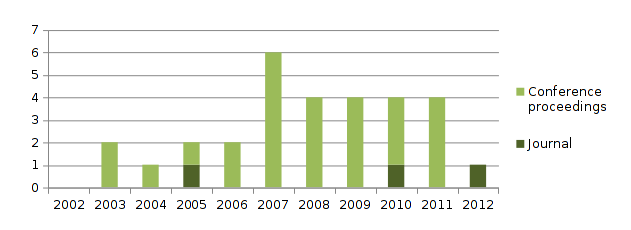
\includegraphics[width=1\textwidth]{img/Publications}
    \caption{Julkaistut tutkimukset vuosittain}
    \label{fig:publications}
  \end{center}
\end{figure}

Suurimmassa osassa julkaisuja oli ilmoitettu ajankohta jolloin muutoksen ensi
askeleet oli otettu. Kuva~\ref{fig:start_year} esittää ilmoitetut muutosten
alkuajankohdat ryhmiteltynä vuosittain. Mediaani muutoksen aloitusajankohdasta
julkaisuvuoteen oli kolme vuotta. Tämä näkyy verrattavasti julkaisujen kasvun
nousussa vuonna 2007 ja aloitettujen muutoshankkeiden nousussa vuonna 2004.
Tästä voidaan päätellä, että suuren mittakaavan muutokset ketteriin menetelmiin
ovat yleistyneet viime vuosikymmenen puolesta välistä alkaen. 

\begin{figure}[htb]
  \begin{center}
    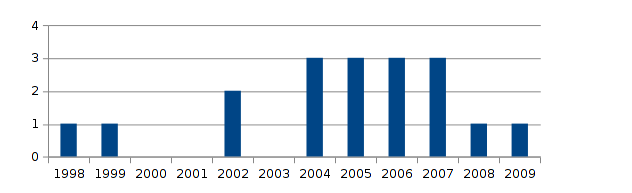
\includegraphics[width=1\textwidth]{img/Transformation_start}
    \caption{Organisaatiomuutosten aloitusajankohdat vuosittain}
    \label{fig:start_year}
  \end{center}
\end{figure}

\subsection{Käytetyt ketterät menetelmät}

Kaikkissa tapauksissa organisaatio oli raportoidun ajanjakson lopussa edelleen
jatkanut ketterien menetelien soveltamista. Muutoksen vaikutuksia oli
tyypillisesti raportoitu 1 tai 2 vuoden päähän sen aloittamisesta. Suurimmassa
osasta tapauksia muutos katsottiin edelleen jatkuvan raportin
kirjoitusajankohtana.

Suurin osa tutkimuksta erotteli käytössä olevia ketteriä menetelmiä.
Taulukko~\ref{table:practices} esittää tutkimuksissa eniten raportoidut
menetelmät. Ylivoimaisesti suosituin ketterä menetelmä oli Scrum, jota
mainittiin käytettävän miltei kahdessa kolmesta organisaatiosta. Toiseksi
suosituin menetelmä oli Extreme Programming. Osassa organisaatioista myös kevyt
kehitysmalli oli yhdistetty ketteriin menetelmiin.

Taulukosta~\ref{table:practices} ilmenee myös eri menetelmien yhdistely
huomattavana trendinä. Lähes kolmanneksessa raporteista mainittiin suoraan, että
menetelmiä oli yhdistelty. Menetelmien yhdistelemistä ja räätälöintiä oli
perusteltu pääasiallisesti kahdella tapaa. Osassa raporteista oli syyksi
mainittu se, että suuren organisaation erityispiirteet tekivät menetelmän
räätälöinnin välttämättömäksi. Toisaalta yritykset olivat halunneet panostaa
mahdollisimman hyvän menetelmän löytämiseen, jolloin useita menetelmiä oli
arvioitu ja niiden sopivimmat piirteet oli yhdistetty.

\begin{table}[h]
    \begin{tabular}{|l|l|}
        \hline
        Menetelmä       & N   \\ \hline
        Scrum           & 18 \\ 
        XP              & 7 \\
        Lean            & 5 \\
        Eri menetelmien yhdistely ja räätälöinti & 9  (epäsuorasti mainittuna useampia) \\
        \hline
    \end{tabular}
	\caption{Hauissa käytetyt näkökulmat ja niitä vastaavat avainsanat. Sarake N
	kuvaa kuinka monessa tutkimuksessa menetelmää mainittiin käytettävän.}
	\label{table:practices}
\end{table}

Edellä mainittujen ketterien mallien lisäksi oli yksittäisiä mainintoja
seuraavista menetelmistä: JAD (Joint Application Development),
ASSF\footnote{Qumer ja Henderson-Sellers [S9] kuvaavat ASSF-menetelmän}, Unified
Process, sekä DSDM (Dynamic Systems Development Method). Näiden menetelmien
lisäksi mainittiin erilaisia käytäntöjä, mukaan lukien ajallinen rytmittäminen,
testivetoinen kehitys, asiakkaan mukanaolo, testauksen automatisointi, sekä
jatkuva yhdentäminen.

\subsection{Perusteet organisaatiomuutoksen aloittamiselle}

\hl{--> Vaatimus parannukseen (16 kpl)}
--> Ongelmia havaittu nykyisessä mallissa (12 kpl)
--> Nopeampi TTM (10 kpl)

\hl{--> Kolmanneksessa tapauksista mainittiin}, että muutokseen ryhdyttiin
erityisesti yrityksen johdon aloitteesta.

\hl{--> Organisaatioiden} lähtötila
--> Kolmannes tutkimuksista raportoi vesiputousmallin olevan käytössä
--> Lähes puolella tutkimuksista ilmoittivat tekevänsä pitkiä (vähimmillään
vuoden mittaisia) julkaisusyklejä.

\subsection{Organisaatiomuutosten piirteet}

Ketterien menetelmien käyttöönottoon tähdänneitä organisaatiomuutoksia
tarkastellaan viidestä eri näkökulmasta, jotka ilmenivät ensisijaisista
tutkimuksista. Ensimämiset näkökulmat ovat tapa jolla muutosta johdettiin ja
malli jolla muutosta toteutettiin. Muut keskeiset näkökulmat ovat
organisaatioiden tekemät sijoitukset organisaatiomuutokseen, miten
yhteisönrakentamisella pyrittiin ankkuroimaan muutosta sekä pilotoinnin käyttö.

\subsubsection{Muutoksen johtaminen}

Organisaation johdolla on keskeinen rooli muutoksessa, mikä näkyy siinä, että
suuressa osassa ensisijaisista tutkimuksista kerrottiin, että johto oli
ensimmäisenä käynnistänyt organisaatiomuutksen. Useassa tapauksessa johto oli
myös vetovastuussa muutoksen läpiviemisestä. Esimerkiksi [S4] mukaan johdon
vahva rooli on tärkeää muutoksen juurruttamiseksi onnistuneesti ja oikean
suunnan säilyttämiseksi, vaikka toteuttava porras on vastuussa uusien
käytäntöjen luomisesta. Toisessa tapauksessa [S11] tuotekehitys oli ottanut
käyttöön ketteriä malleja tiimikohtaisesti, mutta uusien käytäntöjen
yhteensovittaminen ja koordinointi koko organisaation laajuudessa vaati
aloitetta johdon tasolla.

Organisaatiomuutos vaatii tahon jolla on vahvaa halua muutokseen, johtamiskykyä
ja vaikutusvaltaa. Useassa tapauksessa muutoksessa oli yksi keskeinen henkilö,
joka toimi muutoksen mestarina (engl. champion). Muun muassa [S6] esittää kuinka
muutos aloitettiin uuden teknologiajohtajan toimesta, jolla oli kokemusta
aikaisemmista organisaatiomuutoksista. Myös [S1] raportoi muutosta, jossa
muutosta veti yksi asialle omistautunut henkilö. Kyseisessä tapauksesa muutoksen
mestari onnistui juurruttamaan muutoksen siten, että hän pystyi lopuksi
luovuttamaan muutoksen vetovastuun organisaatioon muodostuneelle ketteriä
menetelmiä edistävälle yhteisölle [S1]. Kahdessa tapauksessa organisaatio
palkkasi ulkopuolisen konsultin vetämään muutosta [S5, S30].

Joissakin tapauksissa organisaatiomuutosta ohjasi työryhmä johon oli koottu
useita eri näkökulmia edustavia jäseniä. [S17] kertoo miten muutoksen
koordinointia varten perustettiin projektiryhmä, johon kuului jäseniä muun
muassa ylemmästä johdosta, myynnistä, projektijohdosta, ohjelmistokehityksestä
ja graafisesta suunnittelusta. Poikkiorganisatoorillisen työryhmän tärkeäksi
ominaisuudeksi raportoitiin se, että kaikkien osapuolten näkemyksiä kuullaan ja
vastakkainasetteluita sillataan [S15, S19].


\subsubsection{Muutoksen malli}

Yleisin malli josta ensisijaisissa tutkimukseissa raportoitiin oli ketterien
menetelmien askeleittainen käyttöönotto. Esimerkiksi Pertersen ja Wohlin [S27]
kertovat miten askeleittainen käyttöönotto toteutettiin ottamalla ensiksi
käyttöön pienet tiimit ja tuotteen kehitysjono (engl. product backlog), ja vasta
näiden ollessa toiminnassa siirryttiin soveltamaan muita käytäntöjä kuten
jatkuvaa prosessinparannusta ja päiväpalavereita (engl. stand-up meetings).
Wilby [21] kertoo että ketterä kehityks otettiin ensin käyttöön tiimitasolla,
jonka jälkeen todettiin että pitkän tähtäimen suunnittelu pitää myös muuttaa
ketteräksi. Myös Moore ja Spens [S23] esittävät miten suunnittelu muutettiin
joustavaksi ensin yksittäisten tiimien tasolla, mikä synnytti tarpeen kehittää
tehokkaampia tapoja hallita riippuvuuksiin vaikuttavaia muutoksia ja tiimien
tuotosten yhdentämistä. Pilottiprojektit olivat myös suosittu tapa hallita
askeleittaista käyttöönottoa (katso kohta \ref{subsec:pilotointi}).

Vastakohtana askeleittaiselle käyttöönotolle eräässä organisaatiossa päädyttiin
muuttamaan kaikki kehitystiimit yhdellä kertaa käyttämään ketterää mallia.
Perusteluna yhdellä kertaa toteutetulle käyttöönotolle oli johdon pyrkimys
esittää vahvaa määrätietoisuutta muutoksessa, sekä toimintatapojen pitäminen
yhdenmukaisina. Kerralla toteutettun muutoksen raportoitiin onnistuneen. [S19]

Osassa organisaatioita muutoksen myötä päädyttiin malliin jossa yhdistettiin
aikaisempia toimintatapoja ja ketteryyttä. Esimerkiksi Karlström ja Runeson [S8]
kertovat miten ketterät menetelmät yhdistettiin Stage-Gate malliin, joka
helpotti tiimien välistä koordinointia sekä kommunikaatiota markkinoinnin ja
ylemmän johdon kanssa. Wilbyn [S21] kuvaamassa organisaatiossa alkuperäinen
vuosittainen roadmapping-käytöntö sovitettiin ketteräksi lyhentämällä
suunnitteluväliä neljännesvuoteen, ja ottamalla suunnitteluun mukaan edustajia
kaililta organisaation osa-alueilta.

--> Oleellinen tekijä muutoksen lopputuloksessa oli organisaation muut toiminnot
joiden kanssa ketterät ohjelmistokehitystiimit joutuvat kommunikoimaan.
(13 viitettä ja esimerkkiä)

\subsubsection{Konsultointi, koulutus ja muut muutokseen liittyvät sijoitukset}

Ulkopuolisten konsulttien käyttö oli hyvin tyypillistä, ja siitä oli raportoitu
yli puolessa kaikista ensisijaisista tutkimuksista. Konsultteja käytettiin
neuvomaan muutoksen alussa [???], muutoksen vetämisessä [S5, S30] sekä
koulutuksessa [??, ??, ??, ..]

Koulutus oli keskeisessä osassa muutosta, ja siitä raportoi suuri osa
ensisijaisista tutkimuksista. Koulutus, esimerkkejä -->
--> Keskeisissä rooleissa olevien henkilöiden oma-aloitteinen kouluttautuminen.

Koulutuksen lisäksi tietoutta ketteristä menetelmistä edistettiin muun muassa
erilaisilla työpajoilla, epävirallisilla tapaamisilla ja seminaareilla.
(4 viitettä)

Fyysisten tilojen järjestäminen nousi tärkeäksi seikaksi useassa tapauksessa.
(4 viitettä)

Ketterään malliin siirtyminen vaati myös panostusta uusiin työkaluihin
\hl{(ja automaattisiin testihin ym.)}.
Erityisesti laadunvarmistukseen panostettiin. (5 viitettä)

\subsubsection{Yhteisöllisyyden rakentaminen}

Yhteisöllisyyden rakentamista käsiteltiin tärkeänä asiana suuressa osassa
ensisijaisia tutkimuksia. Yhteisöllisyyden luominen uusien työtapojen ympärille 
on keskeistä muutoksen juurruttamisen kannalta. Agile community (5 viitettä).

--> Community of practice (8 viitettä).

Valmentamista (engl. coaching) voidaan pitää eräänä yhteisöllisyyden muotona.
--> valmentamista sovellettiin .. (9 viitettä). 

\subsubsection{Pilottihankkeiden soveltaminen}
\label{subsec:pilotointi}

--> Pilotoinnin käyttö
--> Positiiviset kokemukset pilotoinnista olivat tärkeitä.
--> Pilotointi nähtiin tapana hallita riskejä [S26]
--> Onnistuneet pilotointihankkeet merkitsivät usein käännekohtaa suurempaan
keterien menetelmien käyttöönottoon.

Useassa organisaatioissa oli tarvetta suorittaa usea pilottiprojekti. Syynä oli
muun muassa se, että projektejen katsottiin eroavan toisistaan, ja tarvittiin
todisteita ketterien menetelmien laaja-alaisesta sovellettavuudesta [S26].

Eräässä tapauksessa [S4] raportoitiin pilotoinnista kriittisessä projektissa
johon ei saanut aiheutua keskeytyksiä. --> Miksi? Varmaan jotta tulee enemmän
''real world'' luottamusta.

\subsubsection{??? Muuta ???}

\hl{--> Lopputuloksena oli ketterien menetelmien} pysyvä käyttöönotto, paitsi [S5]
jossa organisaatio alkoi palautua käyttämään vanhaa menetelmää. Yhdessä
tapauksessa ketterien menetelmien pilottiprojekti keskeytettiin
organisaation yleisen taloustilanteen takia [S26].

\subsection{Ongelmia ketterän kehityksen käyttöönotossa}

Onnistuneen ketterien käyttöönotossa esiintyneitä haasteita listataan viidessä
eri kategoriassa. Ensimmäiseksi käsitellään ongelmia saavuttaa tuki ja
yhtenäinen suunta muutokselle. Toisena kategoriana esitellään organisaatioiden
ongelmia soveltaa ketteriä menetelmiä omassa toiminnassaan. Kolmantena haasteena
listataan väärinymmärryksiä ja soveltumattomia tapoja käyttää ketterää
kehitystä. Neljäntenä kategoriana esitellään haasteita sovittaa ketteriä
menetelmiä toimimaan kaikkien organisaation toimintojen kanssa. Viidentenä
käsitellään haasteita jotka ovat aiheutuneet puutteellisesta resursoinnista ja
varautumisesta muutokseen.

\subsubsection{Organisaation yhtenäinen suuntaaminen muutoksessa}

--> Johdon tuen puute (5 viitettä)
--> Muutosvastarinta (5 viitettä)
--> Liika innokkuus (3 viitettä)

Useassa tapauksessa ketterää muutosta uhkasi vanhan toimintamallin palaaminen.
Eräässä tapauksessa [???] kehittäjät palasivat aikatalulupaineen alla käyttämään
vanhasta mallista tuttuja käytäntöjä. Myös arkkitehtuurilliset
yhdentämisvaikeudet eri osastojen välillä johtivat sopimuspohjaisen menettelyn
paluuseen [???].
(7 viitettä)

\subsubsection{Ketterien mallien sovellettavuus}

Muutamassa tapauksessa ketterä kehitys saatiin toimimaan yksittäisten tiimien
tasolla, mutta ongelmia alkoi esiintyä kun ketterää mallia alettiin soveltaa
laajemmin.
(4 viitettä)

Joissakin organisaatioissa havaittiin että ketterä kehitys ei sovellu kaikkiin
toimintoihin.
(4 viitettä) 

\subsubsection{Uuden mallin väärinymmärtäminen}

Ketterien menetelmien soveltaminen väärin oli yleinen ongelma. Muun muassa jos
Scrum-menetelmästä jätettiin oleellisia käytäntöjä pois alkoi ongelmia
ilmenemään [???].
(9 viitettä)

Joissakin tapauksisa raportoitiin että puuttuva tieto uusista ketteristä
menetelmisjä johti ongelmiin.
(3 viitettä)

\subsubsection{Sovittaminen organisaation muiden toimintojen kanssa}

--> Yhteensopivuusongelmat organisaation muiden toimintojen kanssa. Esimerkiksi
myynti ja HR.
(7 viitettä)

--> Vanhat toimintamallit olivat luoneet pohjan organisaation toiminnalle, ja
vanha toimintamalli ei sopinut yhteen ketterän kehityksen kanssa.
(5 viitettä)

Eräs erityisongelma ketterässä kehityksessä on pitkän aikavälin suunnitelmien
heikko painotus. Liiketoiminnta esittää kuitenkin usein tarpeen ennusteille
tulevasta kehityksestä.
(4 viitettä)

\subsubsection{Puutteellinen varautuminen muutokseen}

--> Valmennuksen puute (5 viitettä)

--> Koulutuksen puute (1 viite)

--> Ketterän koulutuksen tarve kasvoi sitä myötä kun yhä useampi tiimi valmistautui
ketterien menetelmien käyttöönottoon. <Joissakin tapauksissa piti hillitä
käyttöönottoa (?)>

--> Koulutuksen riittämättömyyden takia ketteriä menetelmiä ja niiden keskeisiä
periaatteitä ymmärrettiin väärin. <raportoitu tapauksissa X ja Y> Näissä
tapauksissa koulutuksen lisääminen paransi organisaation toimintaa.

--> Puutteellinen muu resursointi (3 viitettä)

\subsection{Muutosprosessin menestyksen tekijät}

Ensisijaisista tutkimuksista tunnistettiin neljä tekijää jotka edesauttoivat
muutosprosessin menestystä. Ensimmäinen tekijä on organisaation yhdenmukainen
suuntaaminen ja muutoksen johtaminen. Muutoksen suunnitteleminen on toinen
tekijä joka esitellään. Kolmanneksi esitellään hyviä käytäntöjä uuden
toimintatavan soveltamisessa. Neljäntenä tekijänä on riittävä resursointi
muutoksen läpiviemiseen.

\subsubsection{Organisaation yhdensuuntaistaminen ja muutoksen johtaminen}

--> Johdon tuki (5 viitettä)
--> Johdon tulee välttää muutokseen pakottamista (4 viitettä)

--> Muutosta johtavan tahon tulee toiminnallaan lisätä ketterien menetelmien
kannatusta (5 viitettä)

--> Muutosprosessiin on hyvä ottaa mukaan kaikki asianomaiset tahot (7 viitettä)

--> Organisaatiossa suunnan ja tavoitteiden tehokas kommunikointi on keskeinen
menestyksen tekijä. (3 viitettä)

\subsubsection{Muutoksen suunnittelminen ja seuraaminen}

Muutoksessa on oleellista tunnistaa muutoksen tärkeimmät osa-alueet ja keskittyä
niihin ensin. (3 viitettä)

--> Muutoksesta voi tehdä suunnitelman (mikä on hyvä suunnitelma?) (3 viitettä)

--> Muutosta kannattaa tarkkailla, ja toiminnan tehokkuutta mitata (4 viitettä)

\subsubsection{Ketterän menetelmän onnistunut soveltaminen}

--> Suunnittele johdon ja esimiesasemissa olevien henkilöiden tehtävät
(3 viitettä)

--> Toteuttavast portaasta lähtevä menetelmien soveltaminen (4 viitettä).

--> Menetelmien soveltaminen (5 viitettä).

Useassa tapauksesa raportoitiin yhdenmukaisten toimintatapojen eduista.
(8 viitettä)
--> Yhdenmukaisuuden katsottiin oleelliseksi tekijäksi useassa organisaatiossa.
Yhdenmukaisuudella pyrittiin muun muassa vertailukelpoisuuteen eri projektien
välillä [???]. Suuressa organisaatiossa on eri toimintojen välisessä
kommunikaatiossa hyötyä yhteisestä sanastosta [???].

\subsubsection{Muutokseen sijottaminen}

--> Ulkopuolisten resurssien hyödyntäminen. (2 viitettä)

--> Koulutus (6 viitettä)

--> Työkaluihin ja ympäristöön sijoittaminen (2 viitettä)
--> CI ja automaatio (1 viite)

% --------------------------------------------------------------------
\clearpage
\section{Johtopäätökset ja yhteenveto}
\label{sec:johtopaatokset}

--> Muistutus työon tavoitteista (sidoksisuus johdantoon)

--> Yhteenveto tuloksista, ja tulosten merkitys
--> Suositus toimnepiteisiin??

--> Ei vertailtu pienten organisaatioiden ketterään käyttöönottoon.
--> Mitkä olivat erityiset tekijät jotka erosivat
--> Spekulatiivinen vastaus

--> Tulosten soveltuvuus
--> Tutkimuksen arviointi

--> Lisätutkimuskysymyksiä jatkoa varten: käyttöönoton laajuus /
oerganisaatiotyypit / mitkä menetelmät / enemmän perusteita miksi ?? 

--> Jatkotutkimukset
--> Pitää tehdä kirjallisuustutkimus seuraten huolellisesti jotakin
kijallisuustutkimuksen menetelmää. Jotta sain järjestelmällisen
kirjallisuustutkimuksen sovitettua kandidaatintyön laajuuteen jouduin
karsimaan useita oleellisia menetelmään kuuluvia muodollisuuksia.


